\chapter{Data Structures: Objects and Arrays}\label{data}

\epigraphhead[30]{
\epigraph{\hspace*{-.1cm}\itshape``On two occasions I have been asked, `Pray, Mr. Babbage, if you put into the machine wrong figures, will the right answers come out?' [...] I am not able rightly to apprehend the kind of confusion of ideas that could provoke such a question.''}%
{---Charles Babbage, Passages from the Life of a Philosopher (1864)}
}\index{Babbage, Charles}\index{object}\index{data structure}

Numbers, Booleans, and strings are the atoms that \index{data}data structures are built from. Many types of information require more than one atom, though. \emph{Objects} allow us to group values—including other objects—to build more complex structures.

The programs we have built so far have been limited by the fact that they were operating only on simple data types. This chapter will introduce basic data structures. By the end of it, you'll know enough to start writing useful programs.

The chapter will work through a more or less realistic programming example, introducing concepts as they apply to the problem at hand. The example code will often build on functions and bindings that were introduced earlier in the text.

The online coding \index{sandbox}sandbox for the book (\href{https://eloquentjavascript.net/code}{\emph{https://eloquentjavascript.net\slash code}}) provides a way to run code in the context of a specific chapter. If you decide to work through the examples in another environment, be sure to first download the full code for this chapter from the sandbox page.

\section{The weresquirrel}\index{weresquirrel example}\index{lycanthropy}

Every now and then, usually between 8 p.m. and 10 p.m., \index{Jacques}Jacques finds himself transforming into a small furry rodent with a bushy tail.

On one hand, Jacques is quite glad that he doesn't have classic lycanthropy. Turning into a squirrel does cause fewer problems than turning into a wolf. Instead of having to worry about accidentally eating the neighbor (\emph{that} would be awkward), he worries about being eaten by the neighbor's cat. After two occasions where he woke up on a precariously thin branch in the crown of an oak, naked and disoriented, he has taken to locking the doors and windows of his room at night and putting a few walnuts on the floor to keep himself busy.

That takes care of the cat and tree problems. But Jacques would prefer to get rid of his condition entirely. The irregular occurrences of the transformation make him suspect that they might be triggered by something. For a while, he believed that it happened only on days when he had been near oak trees. But avoiding oak trees did not stop the problem.\index{journal}

Switching to a more scientific approach, Jacques has started keeping a daily log of everything he does on a given day and whether he changed form. With this data he hopes to narrow down the conditions that trigger the transformations.

The first thing he needs is a data structure to store this information.

\section{Data sets}\index{data structure!collection}\index{memory!organization}

To work with a chunk of digital data, we'll first have to find a way to represent it in our machine's memory. Say, for example, that we want to represent a \index{collection}collection of the numbers 2, 3, 5, 7, and 11.\index{string}

We could get creative with strings—after all, strings can have any length, so we can put a lot of data into them—and use \lstinline`"2 3 5 7 11"` as our representation. But this is awkward. You'd have to somehow extract the digits and convert them back to numbers to access them.\index{array!creation}\index{[] (array)}

Fortunately, JavaScript provides a data type specifically for storing sequences of values. It is called an \emph{array} and is written as a list of values between \index{square brackets}square brackets, separated by commas.

\begin{lstlisting}
let listOfNumbers = [2, 3, 5, 7, 11];
console.log(listOfNumbers[2]);
// → 5
console.log(listOfNumbers[0]);
// → 2
console.log(listOfNumbers[2 - 1]);
// → 3
\end{lstlisting}
\noindent\index{[] (subscript)}\index{array!indexing}

The notation for getting at the elements inside an array also uses \index{square brackets}square brackets. A pair of square brackets immediately after an expression, with another expression inside of them, will look up the element in the left-hand expression that corresponds to the \emph{\index{index}index} given by the expression in the brackets.\index{zero-based counting}

\label{data.array_indexing}The first index of an array is zero, not one. So the first element is retrieved with \lstinline`listOfNumbers[0]`. Zero-based counting has a long tradition in technology and in certain ways makes a lot of sense, but it takes some getting used to. Think of the index as the amount of items to skip, counting from the start of the array.

\label{data.properties}\section{Properties}\index{Math object}\index{Math.max function}\index{length property!for string}\index{object!property}\index{period character}\index{property!access}

We've seen a few suspicious-looking expressions like \lstinline`myString.length` (to get the length of a string) and \lstinline`Math.max` (the maximum function) in past chapters. These are expressions that access a \emph{property} of some value. In the first case, we access the \lstinline`length` property of the value in \lstinline`myString`. In the second, we access the property named \lstinline`max` in the \lstinline`Math` object (which is a collection of mathematics-related constants and functions).\index{property!access}\index{null}\index{undefined}

Almost all JavaScript values have properties. The exceptions are \lstinline`null` and \lstinline`undefined`. If you try to access a property on one of these nonvalues, you get an error.

\begin{lstlisting}
null.length;
// → TypeError: null has no properties
\end{lstlisting}
\noindent\index{dot character|see{period character}}\index{[] (subscript)}\index{period character}\index{square brackets}\index{computed property}\index{property!access}

The two main ways to access properties in JavaScript are with a dot and with square brackets. Both \lstinline`value.x` and \lstinline`value[x]` access a property on \lstinline`value`—but not necessarily the same property. The difference is in how \lstinline`x` is interpreted. When using a dot, the word after the dot is the literal name of the property. When using square brackets, the expression between the brackets is \emph{evaluated} to get the property name. Whereas \lstinline`value.x` fetches the property of \lstinline`value` named ``x'', \lstinline`value[x]` tries to evaluate the expression \lstinline`x` and uses the result, converted to a string, as the property name.

So if you know that the property you are interested in is called \emph{color}, you say \lstinline`value.color`. If you want to extract the property named by the value held in the binding \lstinline`i`, you say \lstinline`value[i]`. Property names are strings. They can be any string, but the dot notation works only with names that look like valid binding names. So if you want to access a property named \emph{2} or \emph{John Doe}, you must use square brackets: \lstinline`value[2]` or \lstinline`value["John Doe"]`.

The elements in an \index{array}array are stored as the array's properties, using numbers as property names. Because you can't use the dot notation with numbers and usually want to use a binding that holds the index anyway, you have to use the bracket notation to get at them.\index{length property!for array}\index{array!length of}

The \lstinline`length` property of an array tells us how many elements it has. This property name is a valid binding name, and we know its name in advance, so to find the length of an array, you typically write \lstinline`array.length` because that's easier to write than \lstinline`array["length"]`.

\label{data.methods}\section{Methods}\index{function!as property}\index{method}\index{string}

Both string and array objects contain, in addition to the \lstinline`length` property, a number of properties that hold function values.

\begin{lstlisting}
let doh = "Doh";
console.log(typeof doh.toUpperCase);
// → function
console.log(doh.toUpperCase());
// → DOH
\end{lstlisting}
\noindent\index{case conversion}\index{toUpperCase method}\index{toLowerCase method}

Every string has a \lstinline`toUpperCase` property. When called, it will return a copy of the string in which all letters have been converted to uppercase. There is also \lstinline`toLowerCase`, going the other way.\index{this binding}

Interestingly, even though the call to \lstinline`toUpperCase` does not pass any arguments, the function somehow has access to the string \lstinline`"Doh"`, the value whose property we called. How this works is described in \hyperref[object.obj_methods]{Chapter 6}.

Properties that contain functions are generally called \emph{methods} of the value they belong to, as in ``\lstinline`toUpperCase` is a method of a string''.

\label{data.array_methods}This example demonstrates two methods you can use to manipulate arrays:

\begin{lstlisting}
let sequence = [1, 2, 3];
sequence.push(4);
sequence.push(5);
console.log(sequence);
// → [1, 2, 3, 4, 5]
console.log(sequence.pop());
// → 5
console.log(sequence);
// → [1, 2, 3, 4]
\end{lstlisting}
\noindent\index{collection}\index{array}\index{push method}\index{pop method}

The \lstinline`push` method adds values to the end of an array, and the \lstinline`pop` method does the opposite, removing the last value in the array and returning it.\index{data structure!stack}

These somewhat silly names are the traditional terms for operations on a \emph{\index{stack}stack}. A stack, in programming, is a data structure that allows you to push values into it and pop them out again in the opposite order so that the thing that was added last is removed first. These are common in programming—you might remember the function \index{call
stack}call
stack from \hyperref[functions.stack]{the previous chapter}, which is an instance of the same idea.

\section{Objects}\index{journal}\index{weresquirrel example}\index{array}\index{record}

Back to the weresquirrel. A set of daily log entries can be represented as an array. But the entries do not consist of just a number or a string—each entry needs to store a list of activities and a Boolean value that indicates whether Jacques turned into a squirrel or not. Ideally, we would like to group these together into a single value and then put those grouped values into an array of log entries.\index{syntax!object}\index{property!definition}\index{braces!object}\index{\{\} (object)}

Values of the type \emph{\index{object}object} are arbitrary collections of properties. One way to create an object is by using braces as an expression.

\begin{lstlisting}
let day1 = {
  squirrel: false,
  events: ["work", "touched tree", "pizza", "running"]
};
console.log(day1.squirrel);
// → false
console.log(day1.wolf);
// → undefined
day1.wolf = false;
console.log(day1.wolf);
// → false
\end{lstlisting}
\noindent\index{quoting!of object properties}\index{colon character}

Inside the braces, there is a list of properties separated by commas. Each property has a name followed by a colon and a value. When an object is written over multiple lines, indenting it like in the example helps with readability. Properties whose names aren't valid binding names or valid numbers have to be quoted.

\begin{lstlisting}
let descriptions = {
  work: "Went to work",
  "touched tree": "Touched a tree"
};
\end{lstlisting}
\noindent\index{braces!object}

This means that braces have \emph{two} meanings in JavaScript. At the start of a \index{statement}statement, they start a \index{block}block of statements. In any other position, they describe an object. Fortunately, it is rarely useful to start a statement with an object in braces, so the ambiguity between these two is not much of a problem.\index{undefined}

Reading a property that doesn't exist will give you the value \lstinline`undefined`.\index{property!assignment}\index{mutability}\index{= operator}

It is possible to assign a value to a property expression with the \lstinline`=` operator. This will replace the property's value if it already existed or create a new property on the object if it didn't.\index{tentacle (analogy)}\index{property!model of}\index{binding!model of}

To briefly return to our tentacle model of \index{binding}bindings—property bindings are similar. They \emph{grasp} values, but other bindings and properties might be holding onto those same values. You may think of objects as octopuses with any number of tentacles, each of which has a name tattooed on it.\index{delete operator}\index{property!deletion}

The \lstinline`delete` operator cuts off a tentacle from such an octopus. It is a unary operator that, when applied to an object property, will remove the named property from the object. This is not a common thing to do, but it is possible.

\begin{lstlisting}
let anObject = {left: 1, right: 2};
console.log(anObject.left);
// → 1
delete anObject.left;
console.log(anObject.left);
// → undefined
console.log("left" in anObject);
// → false
console.log("right" in anObject);
// → true
\end{lstlisting}
\noindent\index{in operator}\index{property!testing for}\index{object}

The binary \lstinline`in` operator, when applied to a string and an object, tells you whether that object has a property with that name. The difference between setting a property to \lstinline`undefined` and actually deleting it is that, in the first case, the object still \emph{has} the property (it just doesn't have a very interesting value), whereas in the second case the property is no longer present and \lstinline`in` will return \lstinline`false`.\index{Object.keys function}

To find out what properties an object has, you can use the \lstinline`Object.keys` function. You give it an object, and it returns an array of strings—the object's property names.

\begin{lstlisting}
console.log(Object.keys({x: 0, y: 0, z: 2}));
// → ["x", "y", "z"]
\end{lstlisting}
\noindent

There's an \lstinline`Object.assign` function that copies all properties from one object into another.

\begin{lstlisting}
let objectA = {a: 1, b: 2};
Object.assign(objectA, {b: 3, c: 4});
console.log(objectA);
// → {a: 1, b: 3, c: 4}
\end{lstlisting}
\noindent\index{array}\index{collection}

Arrays, then, are just a kind of object specialized for storing sequences of things. If you evaluate \lstinline`typeof []`, it produces \lstinline`"object"`. You can see them as long, flat octopuses with all their tentacles in a neat row, labeled with numbers.\index{journal}\index{weresquirrel example}

We will represent the journal that Jacques keeps as an array of objects.

\begin{lstlisting}
let journal = [
  {events: ["work", "touched tree", "pizza",
            "running", "television"],
   squirrel: false},
  {events: ["work", "ice cream", "cauliflower",
            "lasagna", "touched tree", "brushed teeth"],
   squirrel: false},
  {events: ["weekend", "cycling", "break", "peanuts",
            "beer"],
   squirrel: true},
  /* and so on... */
];
\end{lstlisting}
\noindent

\section{Mutability}

We will get to actual programming \emph{real} soon now. First there's one more piece of theory to understand.\index{mutability}\index{side effect}\index{number}\index{string}\index{Boolean}\index{object!mutability}

We saw that object values can be modified. The types of values discussed in earlier chapters, such as numbers, strings, and Booleans, are all \emph{\index{immutable}immutable}—it is impossible to change values of those types. You can combine them and derive new values from them, but when you take a specific string value, that value will always remain the same. The text inside it cannot be changed. If you have a string that contains \lstinline`"cat"`, it is not possible for other code to change a character in your string to make it spell \lstinline`"rat"`.

Objects work differently. You \emph{can} change their properties, causing a single object value to have different content at different times.\index{object!identity}\index{identity}\index{memory!organization}\index{mutability}

When we have two numbers, 120 and 120, we can consider them precisely the same number, whether or not they refer to the same physical bits. With objects, there is a difference between having two references to the same object and having two different objects that contain the same properties. Consider the following code:

\begin{lstlisting}
let object1 = {value: 10};
let object2 = object1;
let object3 = {value: 10};

console.log(object1 == object2);
// → true
console.log(object1 == object3);
// → false

object1.value = 15;
console.log(object2.value);
// → 15
console.log(object3.value);
// → 10
\end{lstlisting}
\noindent\index{tentacle (analogy)}\index{binding!model of}

The \lstinline`object1` and \lstinline`object2` bindings grasp the \emph{same} object, which is why changing \lstinline`object1` also changes the value of \lstinline`object2`. They are said to have the same \emph{identity}. The binding \lstinline`object3` points to a different object, which initially contains the same properties as \lstinline`object1` but lives a separate life.\index{const keyword}\index{let keyword}\index{binding!as state}

Bindings can also be changeable or constant, but this is separate from the way their values behave. Even though number values don't change, you can use a \lstinline`let` binding to keep track of a changing number by changing the value the binding points at. Similarly, though a \lstinline`const` binding to an object can itself not be changed and will continue to point at the same object, the \emph{contents} of that object might change.

\begin{lstlisting}
const score = {visitors: 0, home: 0};
// This is okay
score.visitors = 1;
// This isn't allowed
score = {visitors: 1, home: 1};
\end{lstlisting}
\noindent\index{== operator}\index{comparison!of objects}\index{deep comparison}

When you compare objects with JavaScript's \lstinline`==` operator, it compares by identity: it will produce \lstinline`true` only if both objects are precisely the same value. Comparing different objects will return \lstinline`false`, even if they have identical properties. There is no ``deep'' comparison operation built into JavaScript, which compares objects by contents, but it is possible to write it yourself (which is one of the \hyperref[data.exercise_deep_compare]{exercises} at the end of this chapter).

\section{The lycanthrope's log}\index{weresquirrel example}\index{lycanthropy}\index{addEntry function}

So, Jacques starts up his JavaScript interpreter and sets up the environment he needs to keep his \index{journal}journal.

\begin{lstlisting}
let journal = [];

function addEntry(events, squirrel) {
  journal.push({events, squirrel});
}
\end{lstlisting}
\noindent\index{braces!object}\index{\{\} (object)}\index{property!definition}

Note that the object added to the journal looks a little odd. Instead of declaring properties like \lstinline`events: events`, it just gives a property name. This is shorthand that means the same thing—if a property name in brace notation isn't followed by a value, its value is taken from the binding with the same name.

So then, every evening at 10 p.m.—or sometimes the next morning, after climbing down from the top shelf of his bookcase—Jacques records the day.

\begin{lstlisting}
addEntry(["work", "touched tree", "pizza", "running",
          "television"], false);
addEntry(["work", "ice cream", "cauliflower", "lasagna",
          "touched tree", "brushed teeth"], false);
addEntry(["weekend", "cycling", "break", "peanuts",
          "beer"], true);
\end{lstlisting}
\noindent

Once he has enough data points, he intends to use statistics to find out which of these events may be related to the squirrelifications.\index{correlation}

\emph{Correlation} is a measure of \index{dependence}dependence between statistical variables. A statistical variable is not quite the same as a programming variable. In statistics you typically have a set of \emph{measurements}, and each variable is measured for every measurement. Correlation between variables is usually expressed as a value that ranges from -1 to 1. Zero correlation means the variables are not related. A correlation of one indicates that the two are perfectly related—if you know one, you also know the other. Negative one also means that the variables are perfectly related but that they are opposites—when one is true, the other is false.\index{phi coefficient}

To compute the measure of correlation between two Boolean variables, we can use the \emph{phi coefficient} (\emph{ϕ}). This is a formula whose input is a \index{frequency table}frequency table containing the number of times the different combinations of the variables were observed. The output of the formula is a number between -1 and 1 that describes the correlation.

We could take the event of eating \index{pizza}pizza and put that in a frequency table like this, where each number indicates the amount of times that combination occurred in our measurements:

\vskip 1.5ex
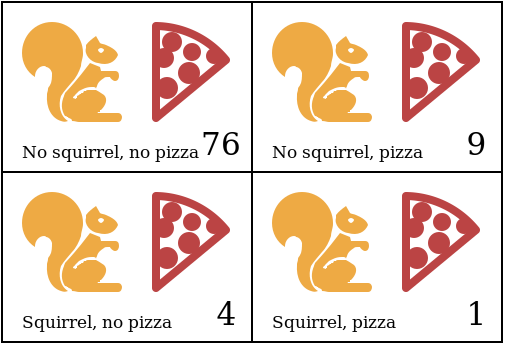
\includegraphics[width=7cm]{img/generated/pizza-squirrel.pdf}
\vskip 1.5ex

If we call that table \emph{n}, we can compute \emph{ϕ} using the following formula:

\begin{equation}\varphi = \frac{n_{11}n_{00}-n_{10}n_{01}}{\sqrt{n_{1\bullet}n_{0\bullet}n_{\bullet1}n_{\bullet0}}}\end{equation}

(If at this point you're putting the book down to focus on a terrible flashback to 10th grade math class—hold on! I do not intend to torture you with endless pages of cryptic notation—it's just this one formula for now. And even with this one, all we do is turn it into JavaScript.)

The notation $n_{01}$ indicates the number of measurements where the first variable (squirrelness) is false (0) and the second variable (pizza) is true (1). In the pizza table, $n_{01}$ is 9.

The value $n_{1\bullet}$ refers to the sum of all measurements where the first variable is true, which is 5 in the example table. Likewise, $n_{\bullet0}$ refers to the sum of the measurements where the second variable is false.\index{correlation}\index{phi coefficient}

So for the pizza table, the part above the division line (the dividend) would be 1×76−4×9 = 40, and the part below it (the divisor) would be the square root of 5×85×10×80, or $\sqrt{340000}$. This comes out to \emph{ϕ} ≈ 0.069, which is tiny. Eating \index{pizza}pizza does not appear to have influence on the transformations.

\section{Computing correlation}\index{array!as table}\index{nesting!of arrays}

We can represent a two-by-two \index{table}table in JavaScript with a four-element array (\lstinline`[76, 9, 4, 1]`). We could also use other representations, such as an array containing two two-element arrays (\lstinline`[[76, 9], [4, 1]]`) or an object with property names like \lstinline`"11"` and \lstinline`"01"`, but the flat array is simple and makes the expressions that access the table pleasantly short. We'll interpret the indices to the array as two-\index{bit}bit \index{binary number}binary numbers, where the leftmost (most significant) digit refers to the squirrel variable and the rightmost (least significant) digit refers to the event variable. For example, the binary number \lstinline`10` refers to the case where Jacques did turn into a squirrel, but the event (say, ``pizza'') didn't occur. This happened four times. And since binary \lstinline`10` is 2 in decimal notation, we will store this number at index 2 of the array.\index{phi coefficient}\index{phi function}

\label{data.phi_function}This is the function that computes the \emph{ϕ} coefficient from such an array:

\begin{lstlisting}
function phi(table) {
  return (table[3] * table[0] - table[2] * table[1]) /
    Math.sqrt((table[2] + table[3]) *
              (table[0] + table[1]) *
              (table[1] + table[3]) *
              (table[0] + table[2]));
}

console.log(phi([76, 9, 4, 1]));
// → 0.068599434
\end{lstlisting}
\noindent\index{square root}\index{Math.sqrt function}

This is a direct translation of the \emph{ϕ} formula into JavaScript. \lstinline`Math.sqrt` is the square root function, as provided by the \lstinline`Math` object in a standard JavaScript environment. We have to add two fields from the table to get fields like $n_{1\bullet}$ because the sums of rows or columns are not stored directly in our data structure.\index{JOURNAL data set}

Jacques kept his journal for three months. The resulting \index{data set}data set is available in the \href{https://eloquentjavascript.net/code#4}{coding sandbox} for this chapter (\href{https://eloquentjavascript.net/code#4}{\emph{https://eloquentjavascript.net\slash code\#4}}), where it is stored in the \lstinline`JOURNAL` binding and in a downloadable \href{https://eloquentjavascript.net/code/journal.js}{file}.\index{tableFor function}

To extract a two-by-two \index{table}table for a specific event from the journal, we must loop over all the entries and tally how many times the event occurs in relation to squirrel transformations.

\begin{lstlisting}
function tableFor(event, journal) {
  let table = [0, 0, 0, 0];
  for (let i = 0; i < journal.length; i++) {
    let entry = journal[i], index = 0;
    if (entry.events.includes(event)) index += 1;
    if (entry.squirrel) index += 2;
    table[index] += 1;
  }
  return table;
}

console.log(tableFor("pizza", JOURNAL));
// → [76, 9, 4, 1]
\end{lstlisting}
\noindent\index{array!searching}\index{includes method}

Arrays have an \lstinline`includes` method that checks whether a given value exists in the array. The function uses that to determine whether the event name it is interested in is part of the event list for a given day.\index{array!indexing}

The body of the loop in \lstinline`tableFor` figures out which box in the table each journal entry falls into by checking whether the entry contains the specific event it's interested in and whether the event happens alongside a squirrel incident. The loop then adds one to the correct box in the table.

We now have the tools we need to compute individual \index{correlation}correlations. The only step remaining is to find a correlation for every type of event that was recorded and see whether anything stands out.

\label{data.for_of_loop}\section{Array loops}\index{for loop}\index{loop}\index{array!iteration}

In the \lstinline`tableFor` function, there's a loop like this:

\begin{lstlisting}
for (let i = 0; i < JOURNAL.length; i++) {
  let entry = JOURNAL[i];
  // Do something with entry
}
\end{lstlisting}
\noindent

This kind of loop is common in classical JavaScript—going over arrays one element at a time is something that comes up a lot, and to do that you'd run a counter over the length of the array and pick out each element in turn.

There is a simpler way to write such loops in modern JavaScript.

\begin{lstlisting}
for (let entry of JOURNAL) {
  console.log(`${entry.events.length} events.`);
}
\end{lstlisting}
\noindent\index{for/of loop}

When a \lstinline`for` loop looks like this, with the word \lstinline`of` after a variable definition, it will loop over the elements of the value given after \lstinline`of`. This works not only for arrays but also for strings and some other data structures. We'll discuss \emph{how} it works in \hyperref[object]{Chapter 6}.

\label{data.analysis}\section{The final analysis}\index{journal}\index{weresquirrel example}\index{journalEvents function}

We need to compute a correlation for every type of event that occurs in the data set. To do that, we first need to \emph{find} every type of event.\index{includes method}\index{push method}

\begin{lstlisting}
function journalEvents(journal) {
  let events = [];
  for (let entry of journal) {
    for (let event of entry.events) {
      if (!events.includes(event)) {
        events.push(event);
      }
    }
  }
  return events;
}

console.log(journalEvents(JOURNAL));
// → ["carrot", "exercise", "weekend", "bread", …]
\end{lstlisting}
\noindent

By going over all the events and adding those that aren't already in there to the \lstinline`events` array, the function collects every type of event.

Using that, we can see all the \index{correlation}correlations.

\begin{lstlisting}
for (let event of journalEvents(JOURNAL)) {
  console.log(event + ":", phi(tableFor(event, JOURNAL)));
}
// → carrot:   0.0140970969
// → exercise: 0.0685994341
// → weekend:  0.1371988681
// → bread:   -0.0757554019
// → pudding: -0.0648203724
// and so on...
\end{lstlisting}
\noindent

Most correlations seem to lie close to zero. Eating carrots, bread, or pudding apparently does not trigger squirrel-lycanthropy. It \emph{does} seem to occur somewhat more often on weekends. Let's filter the results to show only correlations greater than 0.1 or less than -0.1.

\begin{lstlisting}
for (let event of journalEvents(JOURNAL)) {
  let correlation = phi(tableFor(event, JOURNAL));
  if (correlation > 0.1 || correlation < -0.1) {
    console.log(event + ":", correlation);
  }
}
// → weekend:        0.1371988681
// → brushed teeth: -0.3805211953
// → candy:          0.1296407447
// → work:          -0.1371988681
// → spaghetti:      0.2425356250
// → reading:        0.1106828054
// → peanuts:        0.5902679812
\end{lstlisting}
\noindent

Aha! There are two factors with a \index{correlation}correlation that's clearly stronger than the others. Eating \index{peanuts}peanuts has a strong positive effect on the chance of turning into a squirrel, whereas brushing his teeth has a significant negative effect.

Interesting. Let's try something.

\begin{lstlisting}
for (let entry of JOURNAL) {
  if (entry.events.includes("peanuts") &&
     !entry.events.includes("brushed teeth")) {
    entry.events.push("peanut teeth");
  }
}
console.log(phi(tableFor("peanut teeth", JOURNAL)));
// → 1
\end{lstlisting}
\noindent

That's a strong result. The phenomenon occurs precisely when Jacques eats \index{peanuts}peanuts and fails to brush his teeth. If only he weren't such a slob about dental hygiene, he'd have never even noticed his affliction.

Knowing this, Jacques stops eating peanuts altogether and finds that his transformations don't come back.\index{weresquirrel example}

For a few years, things go great for Jacques. But at some point he loses his job. Because he lives in a nasty country where having no job means having no medical services, he is forced to take employment with a \index{circus}circus where he performs as \emph{The Incredible Squirrelman}, stuffing his mouth with peanut butter before every show.

One day, fed up with this pitiful existence, Jacques fails to change back into his human form, hops through a crack in the circus tent, and vanishes into the forest. He is never seen again.

\section{Further arrayology}\index{array!methods}\index{method!array}

Before finishing the chapter, I want to introduce you to a few more object-related concepts. I'll start by introducing some generally useful array methods.\index{push method}\index{pop method}\index{shift method}\index{unshift method}

We saw \lstinline`push` and \lstinline`pop`, which add and remove elements at the end of an array, \hyperref[data.array_methods]{earlier} in this chapter. The corresponding methods for adding and removing things at the start of an array are called \lstinline`unshift` and \lstinline`shift`.

\begin{lstlisting}
let todoList = [];
function remember(task) {
  todoList.push(task);
}
function getTask() {
  return todoList.shift();
}
function rememberUrgently(task) {
  todoList.unshift(task);
}
\end{lstlisting}
\noindent\index{task management example}

That program manages a queue of tasks. You add tasks to the end of the queue by calling \lstinline`remember("groceries")`, and when you're ready to do something, you call \lstinline`getTask()` to get (and remove) the front item from the queue. The \lstinline`rememberUrgently` function also adds a task but adds it to the front instead of the back of the queue.\index{array!searching}\index{indexOf method}\index{lastIndexOf method}

To search for a specific value, arrays provide an \lstinline`indexOf` method. The method searches through the array from the start to the end and returns the index at which the requested value was found—or -1 if it wasn't found. To search from the end instead of the start, there's a similar method called \lstinline`lastIndexOf`.

\begin{lstlisting}
console.log([1, 2, 3, 2, 1].indexOf(2));
// → 1
console.log([1, 2, 3, 2, 1].lastIndexOf(2));
// → 3
\end{lstlisting}
\noindent

Both \lstinline`indexOf` and \lstinline`lastIndexOf` take an optional second argument that indicates where to start searching.\index{slice method}\index{array!indexing}

Another fundamental array method is \lstinline`slice`, which takes start and end indices and returns an array that has only the elements between them. The start index is inclusive, the end index exclusive.

\begin{lstlisting}
console.log([0, 1, 2, 3, 4].slice(2, 4));
// → [2, 3]
console.log([0, 1, 2, 3, 4].slice(2));
// → [2, 3, 4]
\end{lstlisting}
\noindent\index{string!indexing}

When the end index is not given, \lstinline`slice` will take all of the elements after the start index. You can also omit the start index to copy the entire array.\index{concatenation}\index{concat method}

The \lstinline`concat` method can be used to glue arrays together to create a new array, similar to what the \lstinline`+` operator does for strings.

The following example shows both \lstinline`concat` and \lstinline`slice` in action. It takes an array and an index, and it returns a new array that is a copy of the original array with the element at the given index removed.

\begin{lstlisting}
function remove(array, index) {
  return array.slice(0, index)
    .concat(array.slice(index + 1));
}
console.log(remove(["a", "b", "c", "d", "e"], 2));
// → ["a", "b", "d", "e"]
\end{lstlisting}
\noindent

If you pass \lstinline`concat` an argument that is not an array, that value will be added to the new array as if it were a one-element array.

\section{Strings and their properties}\index{string!properties}

We can read properties like \lstinline`length` and \lstinline`toUpperCase` from string values. But if you try to add a new property, it doesn't stick.

\begin{lstlisting}
let kim = "Kim";
kim.age = 88;
console.log(kim.age);
// → undefined
\end{lstlisting}
\noindent

Values of type string, number, and Boolean are not objects, and though the language doesn't complain if you try to set new properties on them, it doesn't actually store those properties. As mentioned earlier, such values are immutable and cannot be changed.\index{string!methods}\index{slice method}\index{indexOf method}\index{string!searching}

But these types do have built-in properties. Every string value has a number of methods. Some very useful ones are \lstinline`slice` and \lstinline`indexOf`, which resemble the array methods of the same name.

\begin{lstlisting}
console.log("coconuts".slice(4, 7));
// → nut
console.log("coconut".indexOf("u"));
// → 5
\end{lstlisting}
\noindent

One difference is that a string's \lstinline`indexOf` can search for a string containing more than one character, whereas the corresponding array method looks only for a single element.

\begin{lstlisting}
console.log("one two three".indexOf("ee"));
// → 11
\end{lstlisting}
\noindent\index{whitespace!trimming}\index{trim method}

The \lstinline`trim` method removes whitespace (spaces, newlines, tabs, and similar characters) from the start and end of a string.

\begin{lstlisting}
console.log("  okay \n ".trim());
// → okay
\end{lstlisting}
\noindent

The \lstinline`zeroPad` function from the \hyperref[functions]{previous chapter} also exists as a method. It is called \lstinline`padStart` and takes the desired length and padding character as arguments.

\begin{lstlisting}
console.log(String(6).padStart(3, "0"));
// → 006
\end{lstlisting}
\noindent

\label{data.split}You can split a string on every occurrence of another string with \lstinline`split` and join it again with \lstinline`join`.

\begin{lstlisting}
let sentence = "Secretarybirds specialize in stomping";
let words = sentence.split(" ");
console.log(words);
// → ["Secretarybirds", "specialize", "in", "stomping"]
console.log(words.join(". "));
// → Secretarybirds. specialize. in. stomping
\end{lstlisting}
\noindent\index{repeat method}

A string can be repeated with the \lstinline`repeat` method, which creates a new string containing multiple copies of the original string, glued together.

\begin{lstlisting}
console.log("LA".repeat(3));
// → LALALA
\end{lstlisting}
\noindent\index{length property!for string}\index{string!indexing}

We have already seen the string type's \lstinline`length` property. Accessing the individual characters in a string looks like accessing array elements (with a caveat that we'll discuss in \hyperref[higher_order.code_units]{Chapter 5}).

\begin{lstlisting}
let string = "abc";
console.log(string.length);
// → 3
console.log(string[1]);
// → b
\end{lstlisting}
\noindent

\label{data.rest_parameters}\section{Rest parameters}\index{Math.max function}

It can be useful for a function to accept any number of \index{argument}arguments. For example, \lstinline`Math.max` computes the maximum of \emph{all} the arguments it is given.\index{period character}\index{max example}\index{spread}

To write such a function, you put three dots before the function's last \index{parameter}parameter, like this:

\begin{lstlisting}
function max(...numbers) {
  let result = -Infinity;
  for (let number of numbers) {
    if (number > result) result = number;
  }
  return result;
}
console.log(max(4, 1, 9, -2));
// → 9
\end{lstlisting}
\noindent

When such a function is called, the \emph{\index{rest parameter}rest parameter} is bound to an array containing all further arguments. If there are other parameters before it, their values aren't part of that array. When, as in \lstinline`max`, it is the only parameter, it will hold all arguments.\index{function!application}

You can use a similar three-dot notation to \emph{call} a function with an array of arguments.

\begin{lstlisting}
let numbers = [5, 1, 7];
console.log(max(...numbers));
// → 7
\end{lstlisting}
\noindent

This ``\index{spread}spreads'' out the array into the function call, passing its elements as separate arguments. It is possible to include an array like that along with other arguments, as in \lstinline`max(9, ...numbers, 2)`.\index{array!of rest arguments}\index{square brackets}

Square bracket array notation similarly allows the triple-dot operator to spread another array into the new array.

\begin{lstlisting}
let words = ["never", "fully"];
console.log(["will", ...words, "understand"]);
// → ["will", "never", "fully", "understand"]
\end{lstlisting}
\noindent

\section{The Math object}\index{Math object}\index{Math.min function}\index{Math.max function}\index{Math.sqrt function}\index{minimum}\index{maximum}\index{square root}

As we've seen, \lstinline`Math` is a grab bag of number-related utility functions, such as \lstinline`Math.max` (maximum), \lstinline`Math.min` (minimum), and \lstinline`Math.sqrt` (square root).\index{namespace}\index{object!property}

\label{data.namespace_pollution}The \lstinline`Math` object is used as a container to group a bunch of related functionality. There is only one \lstinline`Math` object, and it is almost never useful as a value. Rather, it provides a \emph{namespace} so that all these functions and values do not have to be global bindings.\index{binding!naming}

Having too many global bindings ``pollutes'' the namespace. The more names have been taken, the more likely you are to accidentally overwrite the value of some existing binding. For example, it's not unlikely to want to name something \lstinline`max` in one of your programs. Since JavaScript's built-in \lstinline`max` function is tucked safely inside the \lstinline`Math` object, we don't have to worry about overwriting it.\index{let keyword}\index{const keyword}

Many languages will stop you, or at least warn you, when you are defining a binding with a name that is already taken. JavaScript does this for bindings you declared with \lstinline`let` or \lstinline`const` but—perversely—not for standard bindings nor for bindings declared with \lstinline`var` or \lstinline`function`.\index{Math.cos function}\index{Math.sin function}\index{Math.tan function}\index{Math.acos function}\index{Math.asin function}\index{Math.atan function}\index{Math.PI constant}\index{cosine}\index{sine}\index{tangent}\index{PI constant}\index{pi}

Back to the \lstinline`Math` object. If you need to do \index{trigonometry}trigonometry, \lstinline`Math` can help. It contains \lstinline`cos` (cosine), \lstinline`sin` (sine), and \lstinline`tan` (tangent), as well as their inverse functions, \lstinline`acos`, \lstinline`asin`, and \lstinline`atan`, respectively. The number π (pi)—or at least the closest approximation that fits in a JavaScript number—is available as \lstinline`Math.PI`. There is an old programming tradition of writing the names of \index{constant}constant values in all caps.

\begin{lstlisting}
function randomPointOnCircle(radius) {
  let angle = Math.random() * 2 * Math.PI;
  return {x: radius * Math.cos(angle),
          y: radius * Math.sin(angle)};
}
console.log(randomPointOnCircle(2));
// → {x: 0.3667, y: 1.966}
\end{lstlisting}
\noindent

If sines and cosines are not something you are familiar with, don't worry. When they are used in this book, in \hyperref[dom.sin_cos]{Chapter 14}, I'll explain them.\index{Math.random function}\index{random number}

The previous example used \lstinline`Math.random`. This is a function that returns a new pseudorandom number between zero (inclusive) and one (exclusive) every time you call it.

\begin{lstlisting}
console.log(Math.random());
// → 0.36993729369714856
console.log(Math.random());
// → 0.727367032552138
console.log(Math.random());
// → 0.40180766698904335
\end{lstlisting}
\noindent\index{pseudorandom number}\index{random number}

Though computers are deterministic machines—they always react the same way if given the same input—it is possible to have them produce numbers that appear random. To do that, the machine keeps some hidden value, and whenever you ask for a new random number, it performs complicated computations on this hidden value to create a new value. It stores a new value and returns some number derived from it. That way, it can produce ever new, hard-to-predict numbers in a way that \emph{seems} random.\index{rounding}\index{Math.floor function}

If we want a whole random number instead of a fractional one, we can use \lstinline`Math.floor` (which rounds down to the nearest whole number) on the result of \lstinline`Math.random`.

\begin{lstlisting}
console.log(Math.floor(Math.random() * 10));
// → 2
\end{lstlisting}
\noindent

Multiplying the random number by 10 gives us a number greater than or equal to 0 and below 10. Since \lstinline`Math.floor` rounds down, this expression will produce, with equal chance, any number from 0 through 9.\index{Math.ceil function}\index{Math.round function}\index{Math.abs function}\index{absolute value}

There are also the functions \lstinline`Math.ceil` (for ``ceiling'', which rounds up to a whole number), \lstinline`Math.round` (to the nearest whole number), and \lstinline`Math.abs`, which takes the absolute value of a number, meaning it negates negative values but leaves positive ones as they are.

\section{Destructuring}\index{phi function}

Let's go back to the \lstinline`phi` function for a moment.

\begin{lstlisting}
function phi(table) {
  return (table[3] * table[0] - table[2] * table[1]) /
    Math.sqrt((table[2] + table[3]) *
              (table[0] + table[1]) *
              (table[1] + table[3]) *
              (table[0] + table[2]));
}
\end{lstlisting}
\noindent\index{destructuring binding}\index{parameter}

One of the reasons this function is awkward to read is that we have a binding pointing at our array, but we'd much prefer to have bindings for the \emph{elements} of the array, that is, \lstinline`let n00 = table[0]` and so on. Fortunately, there is a succinct way to do this in JavaScript.

\begin{lstlisting}
function phi([n00, n01, n10, n11]) {
  return (n11 * n00 - n10 * n01) /
    Math.sqrt((n10 + n11) * (n00 + n01) *
              (n01 + n11) * (n00 + n10));
}
\end{lstlisting}
\noindent\index{let keyword}\index{var keyword}\index{const keyword}\index{binding!destructuring}

This also works for bindings created with \lstinline`let`, \lstinline`var`, or \lstinline`const`. If you know the value you are binding is an array, you can use \index{square brackets}square brackets to ``look inside'' of the value, binding its contents.\index{object!property}\index{braces!object}

A similar trick works for objects, using braces instead of square brackets.

\begin{lstlisting}
let {name} = {name: "Faraji", age: 23};
console.log(name);
// → Faraji
\end{lstlisting}
\noindent\index{null}\index{undefined}

Note that if you try to destructure \lstinline`null` or \lstinline`undefined`, you get an error, much as you would if you directly try to access a property of those values.

\section{JSON}\index{array!representation}\index{object!representation}\index{data format}\index{memory!organization}

Because properties only grasp their value, rather than contain it, objects and arrays are stored in the computer's memory as sequences of bits holding the \emph{\index{address}addresses}—the place in memory—of their contents. So an array with another array inside of it consists of (at least) one memory region for the inner array, and another for the outer array, containing (among other things) a binary number that represents the position of the inner array.

If you want to save data in a file for later or send it to another computer over the network, you have to somehow convert these tangles of memory addresses to a description that can be stored or sent. You \emph{could} send over your entire computer memory along with the address of the value you're interested in, I suppose, but that doesn't seem like the best approach.\index{JavaScript Object Notation|see{JSON}}\index{serialization}\index{World Wide Web}

What we can do is \emph{serialize} the data. That means it is converted into a flat description. A popular serialization format is called \emph{\index{JSON}JSON} (pronounced ``Jason''), which stands for JavaScript Object Notation. It is widely used as a data storage and communication format on the Web, even in languages other than JavaScript.\index{array!notation}\index{object!creation}\index{quoting!in JSON}\index{comment}

JSON looks similar to JavaScript's way of writing arrays and objects, with a few restrictions. All property names have to be surrounded by double quotes, and only simple data expressions are allowed—no function calls, bindings, or anything that involves actual computation. Comments are not allowed in JSON.

A journal entry might look like this when represented as JSON data:

\begin{lstlisting}
{
  "squirrel": false,
  "events": ["work", "touched tree", "pizza", "running"]
}
\end{lstlisting}
\noindent\index{JSON.stringify function}\index{JSON.parse function}\index{serialization}\index{deserialization}\index{parsing}

JavaScript gives us the functions \lstinline`JSON.stringify` and \lstinline`JSON.parse` to convert data to and from this format. The first takes a JavaScript value and returns a JSON-encoded string. The second takes such a string and converts it to the value it encodes.

\begin{lstlisting}
let string = JSON.stringify({squirrel: false,
                             events: ["weekend"]});
console.log(string);
// → {"squirrel":false,"events":["weekend"]}
console.log(JSON.parse(string).events);
// → ["weekend"]
\end{lstlisting}
\noindent

\section{Summary}

Objects and arrays (which are a specific kind of object) provide ways to group several values into a single value. Conceptually, this allows us to put a bunch of related things in a bag and run around with the bag, instead of wrapping our arms around all of the individual things and trying to hold on to them separately.

Most values in JavaScript have properties, the exceptions being \lstinline`null` and \lstinline`undefined`. Properties are accessed using \lstinline`value.prop` or \lstinline`value["prop"]`. Objects tend to use names for their properties and store more or less a fixed set of them. Arrays, on the other hand, usually contain varying amounts of conceptually identical values and use numbers (starting from 0) as the names of their properties.

There \emph{are} some named properties in arrays, such as \lstinline`length` and a number of methods. Methods are functions that live in properties and (usually) act on the value they are a property of.

You can iterate over arrays using a special kind of \lstinline`for` loop—\lstinline`for (let element of array)`.

\section{Exercises}

\subsection{The sum of a range}\index{summing (exercise)}

The \hyperref[intro]{introduction} of this book alluded to the following as a nice way to compute the sum of a range of numbers:

\begin{lstlisting}
console.log(sum(range(1, 10)));
\end{lstlisting}
\noindent\index{range function}\index{sum function}

Write a \lstinline`range` function that takes two arguments, \lstinline`start` and \lstinline`end`, and returns an array containing all the numbers from \lstinline`start` up to (and including) \lstinline`end`.

Next, write a \lstinline`sum` function that takes an array of numbers and returns the sum of these numbers. Run the example program and see whether it does indeed return 55.\index{optional argument}

As a bonus assignment, modify your \lstinline`range` function to take an optional third argument that indicates the ``step'' value used when building the array. If no step is given, the elements go up by increments of one, corresponding to the old behavior. The function call \lstinline`range(1, 10, 2)` should return \lstinline`[1, 3, 5, 7, 9]`. Make sure it also works with negative step values so that \lstinline`range(5, 2, -1)` produces \lstinline`[5, 4, 3, 2]`.

\subsection{Reversing an array}\index{reversing (exercise)}\index{reverse method}\index{array!methods}

Arrays have a \lstinline`reverse` method that changes the array by inverting the order in which its elements appear. For this exercise, write two functions, \lstinline`reverseArray` and \lstinline`reverseArrayInPlace`. The first, \lstinline`reverseArray`, takes an array as argument and produces a \emph{new} array that has the same elements in the inverse order. The second, \lstinline`reverseArrayInPlace`, does what the \lstinline`reverse` method does: it \emph{modifies} the array given as argument by reversing its elements. Neither may use the standard \lstinline`reverse` method.\index{efficiency}\index{pure function}\index{side effect}

Thinking back to the notes about side effects and pure functions in the \hyperref[functions.pure]{previous chapter}, which variant do you expect to be useful in more situations? Which one runs faster?

\label{data.list}\subsection{A list}\index{data structure!list}\index{list (exercise)}\index{linked list}\index{array}\index{collection}

Objects, as generic blobs of values, can be used to build all sorts of data structures. A common data structure is the \emph{list} (not to be confused with array). A list is a nested set of objects, with the first object holding a reference to the second, the second to the third, and so on.

\begin{lstlisting}
let list = {
  value: 1,
  rest: {
    value: 2,
    rest: {
      value: 3,
      rest: null
    }
  }
};
\end{lstlisting}
\noindent

The resulting objects form a chain, like this:

\vskip 1.5ex
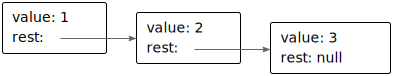
\includegraphics[width=8cm]{img/generated/linked-list.pdf}
\vskip 1.5ex\index{structure sharing}\index{memory!structure!sharing}

A nice thing about lists is that they can share parts of their structure. For example, if I create two new values \lstinline`{value: 0, rest: list}` and \lstinline`{value: -1, rest: list}` (with \lstinline`list` referring to the binding defined earlier), they are both independent lists, but they share the structure that makes up their last three elements. The original list is also still a valid three-element list.

Write a function \lstinline`arrayToList` that builds up a list structure like the one shown when given \lstinline`[1, 2, 3]` as argument. Also write a \lstinline`listToArray` function that produces an array from a list. Then add a helper function \lstinline`prepend`, which takes an element and a list and creates a new list that adds the element to the front of the input list, and \lstinline`nth`, which takes a list and a number and returns the element at the given position in the list (with zero referring to the first element) or \lstinline`undefined` when there is no such element.\index{recursion}

If you haven't already, also write a recursive version of \lstinline`nth`.

\label{data.exercise_deep_compare}\subsection{Deep comparison}\index{deep comparison (exercise)}\index{comparison!deep}\index{deep comparison}\index{== operator}

The \lstinline`==` operator compares objects by identity. But sometimes you'd prefer to compare the values of their actual properties.

Write a function \lstinline`deepEqual` that takes two values and returns true only if they are the same value or are objects with the same properties, where the values of the properties are equal when compared with a recursive call to \lstinline`deepEqual`.\index{null}\index{=== operator}\index{typeof operator}

To find out whether values should be compared directly (use the \lstinline`===` operator for that) or have their properties compared, you can use the \lstinline`typeof` operator. If it produces \lstinline`"object"` for both values, you should do a deep comparison. But you have to take one silly exception into account: because of a historical accident, \lstinline`typeof null` also produces \lstinline`"object"`.\index{Object.keys function}

The \lstinline`Object.keys` function will be useful when you need to go over the properties of objects to compare them.
